\documentclass[../Bachelorarbeit.tex]{subfiles}
\begin{document}

\subsection{Anwendungsfallspezifikation} \label{AnwfallSpez}
Nach dem Abschließen der Festlegung des Kontextes des mehrachsigen Positioniersystems folgt nun die Identifizierung von Systemprozessen. Der Findungsprozess erfolgt über die Anwendungsfallanalyse. Dabei wird ein System als Black-Box betrachtet, um möglichst gute Systemprozesse zu finden, ohne sich von internen Gegebenheiten des Systems beeinflussen zu lassen.\\ % Quelle
Die Anwendungsfallspezifikation wird in dieser Arbeit in zwei Unterkapitel eingeteilt. Ersteres beschäftigt sich mit dem Finden und Entwickeln von Systemprozessen. Das zweite Unterkapitel hat zum Ziel die Systemprozesse zu präzisieren und diese dann übersichtlich darzustellen.\\

\subsubsection{Entwicklung der Systemprozesse}
Die Anwendungsfallanalyse baut auf dem Anwendungsfalldiagramm aus \autoref{fig:my-img1} auf. Dabei findet auch an dieser Stelle eine Unterteilung in zwei Abschnitte statt. Im ersten Schritt werden die Akteure aus den Diagrammen des \autoref{kontextana} geprüft und um eventuelle Akteure ergänzt, die bis zu diesem Zeitpunkt nicht erkannt wurden. Diese werden zunächst in die Kontextabgrenzung mit aufgenommen, bevor im folgenden Abschnitt die Anwendungsfallanalyse beginnt.\\
Im zweiten Schritt werden die Erwartungen der Akteue an das System untersucht. Aus dieser Analyse erfolgt die Ableitunge von möglichen Systemprozessen. Dieser Abschnitt hat es folglich als Ziel, die Frage nach den durch die Akteure geforderten Voraussetzungen zu beantworten.\\
Für die Entwicklung der Systemprozzesse wird folglich auf den logischen Kontext zurückgegriffen, da dieser die Akteure des Systems bereits im Anwendungsfalldiagramm (siehe \autoref{fig:my-img1}) zeigt. Da es nur um die Frage nach den Akteuren und ihren Erwartungen geht und dabei die Hardware und die Ausprägung der Kommunikation des Positioniersystems nicht relevant ist, spielen der physikalische Kontext und dessen Ergebnisse keine Rolle.\\
Die \autoref{fig:my-img3} zeigt die Systemprozesse, die aus der Anlagenbeschreibung modelliert werden. Es ist ersichtlich, dass gezeigtes Anwendungsfalldiagramm eine Erweiterung der \autoref{fig:my-img1} aus dem vorhergegangenen Unterabschnitt ist.\\
Neu daszugekommen sind die Anwendungsfälle, die durch den Anlagennutzer ausgelöst werden können. Konkret handelt es sich also um die zwei auswählbaren Betriebsmodi und den Not-Halt. Weiterhin ist der Transport von Gegenständen im Anwendungsfalldiagramm aufgeführt. Es handelt sich dabei um den grundsätzlichen Nutzen des Positioniersystems. Es ist wichtig zu berücksichtigen, dass dieser Anwendungsfall von den vorher genannten drei Anwendungsfällen/Betriebszuständen abhängig ist. Zuletzt findet sich noch die Bereitstellung von Prozessdaten im Diagramm wieder.

\begin{figure}[h]
    \centering
    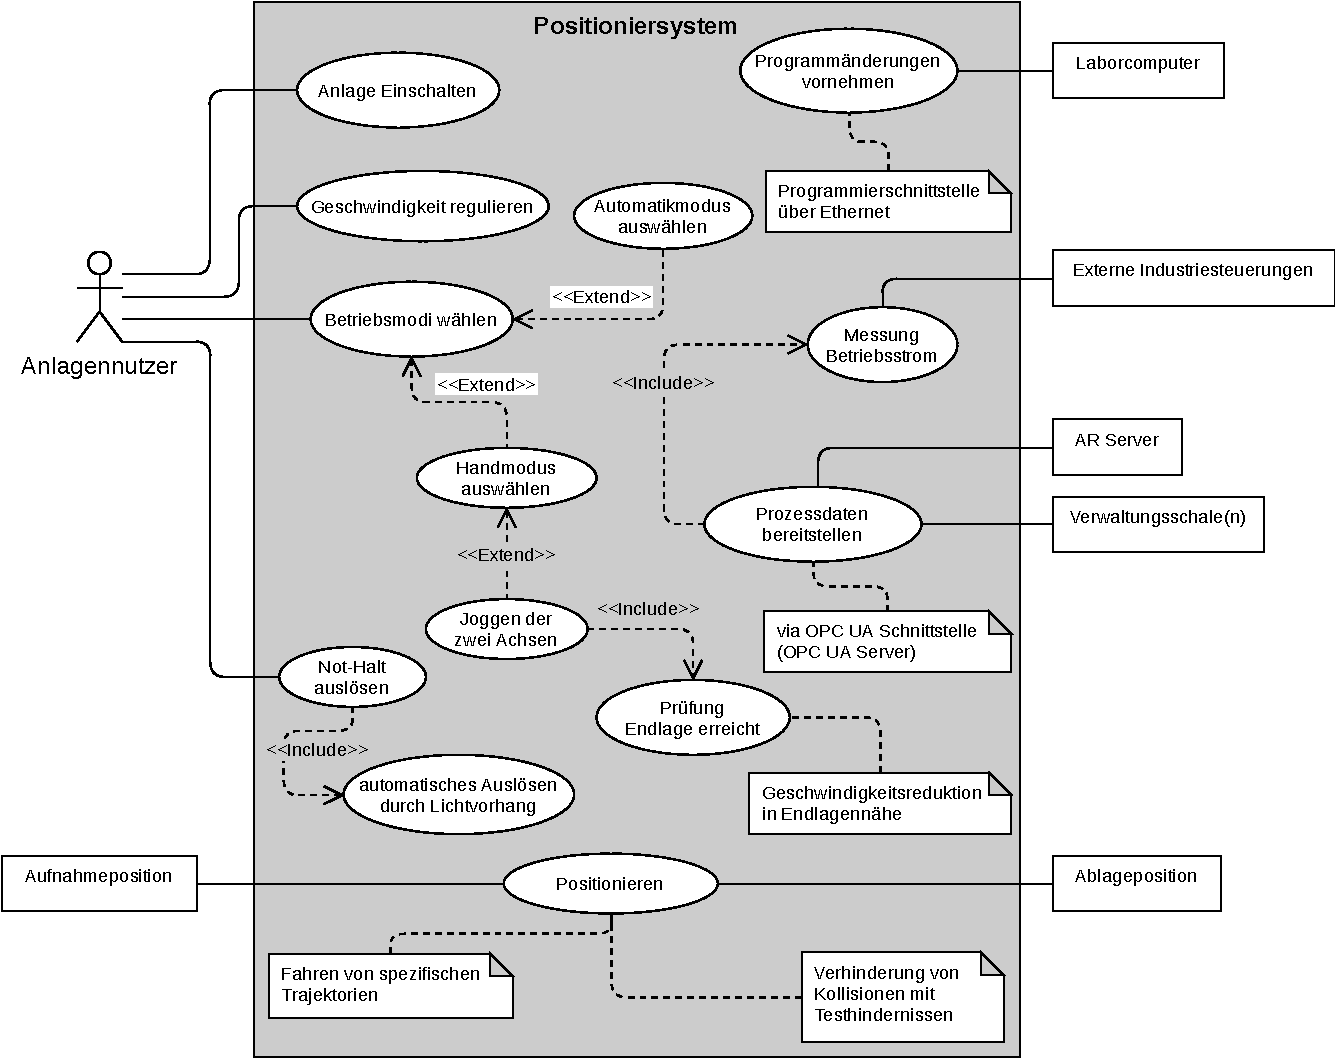
\includegraphics[width=\textwidth]{Images/use_case_dia.pdf}
    \caption[Anwendungsfalldiagramm]{Anwendungsfalldiagramm des Positioniersystems}
    \label{fig:my-img3}
\end{figure}

\subsubsection{Präzisierung der Systemprozesse} \label{AnwfallSpezPraez}
Dieser Unterabschnitt greift die Systemprozesse aus der Anwendungsfallanalyse des vorhergegangenen Unterabschnittes noch einmal auf und verfeinert diese. Im Folgenden wird zunächst die genutzte Methodik zur spezifizierung der Systemeprozesse vorgestellt.\\
Für die Spezifikation von Systemprozessen empfiehlt es sich die Anwendungsfallbeschreibung als Mittel zur Dokumentation zu nutzen. Diese sollte in Form von Tabellen erfolgen. Dabei wird jeder einzelne Akteur in seiner eigenen Tabelle dargestellt. Bei den relevanten Tabelleneinträgen handelt es sich um die Zeilen Name, Akteur, auslösendes Ereignis, Kurzbeschreibung, Vorbedingungen, essenzielle Schritte, Ausnahmefälle, Nachbedingungen, Zeitverhalten, Verfügbarkeit und Kommentare/Fragen.\\ % Quelle
Sowohl der \textbf{Name} als auch der \textbf{Akteur} wird dabei aus dem Anwendungsfalldiagramm aus \autoref{fig:my-img3} übernommen. Es sind am Ende alle Akteure aus dem Anwendungsfalldiagramm tabellarisch aufgenommen. Das Feld \textbf{auslösendes Ereignis} beschreibt den Initiator des Anwendungsfalls. Der nächste Eintrag, die \textbf{Kurzbeschreibung} ist eine in zwei bis vier Sätzen dokumentierte wörtliche Beschreibung des Prozesses und dient zur Darstellung seines Kerns. Das Feld \textbf{Vorbedingungen} enthält zusammengefasst alle Voraussetzungen, die für die Ausführung des Anwendungsfalls nötig sind. Der nächste Eintrag stellt den wichtigsten Schritt in der Dokumentation des Anwendungsfalls dar. Dieser wird unterteilt in zwei weitere Felder, die im direkten Bezug zueinander stehen. Es werden Auf der einen Seite Ereignisse aufgenommen, die während der Standardausführung des Prozesses auftreten \bzw. auftreten können und auf der anderen Seite die Reaktionen des Systems auf diese Ereignisse. Das Feld \textbf{Ausnahmefälle} betrachtet alle Fehler und Ausnahmesituationen, die Abweichend von der Standardausführung auftreten können. Die \textbf{Nachbedingungen} sind analog zu den Vorbedingungen zu dokumentieren und beschreiben den Endzustand des Prozesses nach einer Standardausführung. In den Punkten \textbf{Zeitverhalten} und \textbf{Verfügbarkeit} können \acp{nfa} des Anwendungsfalls festgehalten werden. Zuletzt, im Feld \textbf{Kommentare/Fragen}, können Anmerkungen und Probleme aufgenommen werden, falls diese existieren. Es gilt diese bis zur Fertigstellung des Systems zu eliminieren, so dass dieses Feld leer bleiben kann. Es handelt sich folglich um ein temporäres Hilsmittel.\\
Es bietet sich im Normallfall an zwei Abstraktionsebenen in der Darstellung der Systemprozesse zu nutzen. Dazu gehört eine detaillierte Dokumentation für die Prozessentwickler und ein abstrahierter Überblick für Manager und weniger stark involvierte Personen. Auf dieses Überblick wird jedoch an dieser Stelle verzichtet, da alle für das System relevanten Personen und Stakeholder ausreichend mit der Positioniereinheit und der Umsetzung eines solchen Systems vertraut sind. Im Anhang kann jedoch trotzdem zu jedem Akteur auch ein Überblick gefunden werden.\\
Es folgen nun die tabellarischen Darstellungen zu den Anwendungsfällen nach beschriebenem Muster.\\

\begin{longtable}[c]{| p{0.28\linewidth} | p{0.32\linewidth} | p{0.32\linewidth} |}
    \hline
    \textbf{Name}                   &   \multicolumn{2}{| l |}{Objekt transportieren}                                      \\ \hline
    \textbf{Akteur}                 &   \multicolumn{2}{| l |}{Aufnahmeposition}                                            \\ \hline
    \textbf{Auslösendes Ereignis}   &   \multicolumn{2}{| l |}{Ein neues Transportobjeckt liegt auf Aufnahmeposition bereit}    \\ \hline
    \textbf{Kurzbeschreibung}       &   \multicolumn{2}{|p{\dimexpr0.64\linewidth+4\tabcolsep}|}{Das Objekt wird mit einem Greifer von der Aufnahmeposition hochgenommen. Anschließend fährt das Positioniersystem eine Hindernissausweichende Trajektorie zur Ablageposition. Dort wird das Objekt wieder losgelassen.}                                                                                                    \\ \hline
    \textbf{Vorbedingungen}         &   \multicolumn{2}{|p{\dimexpr0.64\linewidth+4\tabcolsep}|}{\begin{itemize}[noitemsep,topsep=0pt,parsep=0pt,partopsep=0pt,leftmargin=*]
                                                                    \item der Automatikmodus wurde ausgewählt
                                                                    \item Aufnahmeschale ist mit Transportobjekt bestückt
                                                                \end{itemize}}       \\ \hline
    \multirow{6}{=}{\textbf{Essenzielle Schritte}}  &   \textbf{Intention der Systemumgebung}   &   \textbf{Reaktion des Systems}   \\ \cline{2-3}
                                                    &   Anlagennutzer will das System einschalten   &   Systemkomponenten werden mit Spannung versorgt und sind betriebsbereit  \\ \cline{2-3}
                                                    &   Anlagennutzer will, dass die Positioniereinheit vollautomatisch Transportgüter von der Aufnahmeposition zur Ablageposition befördert    &   Laboranlage beginnt Objekte von der Aufnahmeposition zu greifen und zu transportieren   \\ \cline{2-3}
                                                    &   Anlagennutzer will das System auf Grund einer Gefahrensituation anhalten    &   Die Laboranlage bremst bis zum Stillstand ab und erwartet eine Bestätigung, dass die Gefahren- \bzw Fehlersituation beseitigt ist   \\ \cline{2-3}
                                                    &   Anlagennutzer will die Fahrgeschwindigkeit regulieren   &   Die Achsen des Systems bewegen sich entsprechend der analogen Nutzereingabe schneller \bzw langsamer \\ \cline{2-3}
                                                    &   Anlagennutzer will die Laboranlage stoppen  &   Der Automatikbetrieb beendet seinen aktiven Zyklus und wird dann abgewählt, woraufhin die Anlage stoppt  \\ \hline
    \textbf{Ausnahmefälle}          &   \multicolumn{2}{|p{\dimexpr0.64\linewidth+4\tabcolsep}|}{\begin{itemize}[noitemsep,topsep=0pt,parsep=0pt,partopsep=0pt,leftmargin=*]
                                            % \item Sicherheitsbedingtes Auslösen der Not-Halt Funktionalität
                                            \item Defektbedingte Abschaltung der Anlage
                                        \end{itemize}}                                                                  \\ \hline
    \textbf{Nachbedingungen}        &   \multicolumn{2}{|p{\dimexpr0.64\linewidth+4\tabcolsep}|}{Der Automatikmodus ist beendet und die Anlage kann abgeschaltet werden.}                                     \\ \hline
    \textbf{Zeitverhalten}          &   \multicolumn{2}{| l |}{schnell und effizient}                                       \\ \hline
    \textbf{Verfügbarkeit}          &   \multicolumn{2}{| l |}{maximal ein Systemausfall in 10.000h}                        \\ \hline
    \textbf{Kommentare/Fragen}      &   \multicolumn{2}{| l |}{-\xspace -\xspace -}                                         \\ \hline
    
    \caption[Systemprozess - Objekttransport]{Anwendungsfallbeschreibung - Systemprozess: Objekttransport}
    \label{tab:my-table41} 
\end{longtable}

\begin{longtable}[c]{| p{0.28\linewidth} | p{0.32\linewidth} | p{0.32\linewidth} |}
    \hline
    \textbf{Name}                   &   \multicolumn{2}{| l |}{manuelle Funktionsausführung}                                      \\ \hline
    \textbf{Akteur}                 &   \multicolumn{2}{| l |}{Anlagennutzer}                                            \\ \hline
    \textbf{Auslösendes Ereignis}   &   \multicolumn{2}{|p{\dimexpr0.64\linewidth+4\tabcolsep}|}{Der Vierwegetaster oder die Greifertaster an der Schaltschrankfront werden betätigt}    \\ \hline
    \textbf{Kurzbeschreibung}       &   \multicolumn{2}{|p{\dimexpr0.64\linewidth+4\tabcolsep}|}{Die dem betätigten Taster zugehörige Achse bewegt sich entsprechend der angezeigten Richtung auf diesem Taster. Wird einer der dem Greider zugehörigen Taster gedrückt, Schwenkt der Greeifarm um \bzw der Greifer öffnet/schließt}                                                                                                    \\ \hline
    \textbf{Vorbedingungen}         &   \multicolumn{2}{|p{\dimexpr0.64\linewidth+4\tabcolsep}|}{\begin{itemize}[noitemsep,topsep=0pt,parsep=0pt,partopsep=0pt,leftmargin=*]
                                                                    \item der Handmodus wurde ausgewählt
                                                                    \item mindestens einer der vier Richtungstaster auf dem Vierwegetaster wird gedrückt oder einer der beiden dem Greifer zugehörigen Taster
                                                                \end{itemize}}       \\ \hline
    \multirow{9}{=}{\textbf{Essenzielle Schritte}}  &   \textbf{Intention der Systemumgebung}   &   \textbf{Reaktion des Systems}   \\ \cline{2-3}
                                                    &   Anlagennutzer will das System einschalten   &   Systemkomponenten werden mit Spannung versorgt und sind betriebsbereit  \\ \cline{2-3}
                                                    &   Anlagennutzer will auf der horizontalen Achse positionieren   &   Das Positioniersystem erwartet Tastereingabe, die zum Joggen der X-Achse führt \\ \cline{2-3}
                                                    &   Anlagennutzer will auf der vertikalen Achse positionieren   &   Das Positioniersystem erwartet Tastereingabe, die zum Joggen der Z-Achse führt \\ \cline{2-3}
                                                    &   Anlagennutzer will den Greifarm umschwenken   &   Das Positioniersystem erwartet Tastereingabe, die zum Schwenken des Greifarms führt \\ \cline{2-3}
                                                    &   Anlagennutzer will ein Objekt greifen loslassen  &   Das Positioniersystem erwartet Tastereingabe, die zum Öffen \bzw Schließen des Greifers führt \\ \cline{2-3}
                                                    &   Anlagennutzer will das System auf Grund einer Gefahrensituation anhalten    &   Die Laboranlage bremst bis zum Stillstand ab und erwartet eine Bestätigung, dass die Gefahren- \bzw Fehlersituation beseitigt ist   \\ \cline{2-3}
                                                    &   Anlagennutzer will die Fahrgeschwindigkeit regulieren   &   Die Achsen des Systems bewegen sich entsprechend der analogen Nutzereingabe schneller \bzw langsamer \\ \cline{2-3}
                                                    &   Anlagennutzer will die Laboranlage stoppen  &   Die Anlage ist gestoppt und der Handmodus wird abgewählt  \\ \hline
    \textbf{Ausnahmefälle}          &   \multicolumn{2}{|p{\dimexpr0.64\linewidth+4\tabcolsep}|}{\begin{itemize}[noitemsep,topsep=0pt,parsep=0pt,partopsep=0pt,leftmargin=*]
                                            % \item Sicherheitsbedingtes Auslösen der Not-Halt Funktionalität
                                            \item Defektbedingte Abschaltung der Anlage
                                        \end{itemize}}                                                                  \\ \hline
    \textbf{Nachbedingungen}        &   \multicolumn{2}{| l |}{Anlage ist abgeschaltet}                                     \\ \hline
    \textbf{Zeitverhalten}          &   \multicolumn{2}{|p{\dimexpr0.64\linewidth+4\tabcolsep}|}{Keine Ansprüche an das Zeitverhalten (Handmodus wird nur zu Testzwecken genutzt)}                                       \\ \hline
    \textbf{Verfügbarkeit}          &   \multicolumn{2}{| l |}{maximal ein Systemausfall in 10.000h}                        \\ \hline
    \textbf{Kommentare/Fragen}      &   \multicolumn{2}{| l |}{-\xspace -\xspace -}                                         \\ \hline
    
    \caption[Systemprozess - manuelle Funktionsausführung]{Anwendungsfallbeschreibung - Systemprozess: manuelle Funktionsausführung}
    \label{tab:my-table42} 
\end{longtable}

\begin{longtable}[c]{| p{0.28\linewidth} | p{0.32\linewidth} | p{0.32\linewidth} |}
    \hline
    \textbf{Name}                   &   \multicolumn{2}{| l |}{Programmänderungen Vornehmen}                                      \\ \hline
    \textbf{Akteur}                 &   \multicolumn{2}{| l |}{Laborcomputer}                                            \\ \hline
    \textbf{Auslösendes Ereignis}   &   \multicolumn{2}{| l |}{System wird mit neuem Programmcode bespielt}    \\ \hline
    \textbf{Kurzbeschreibung}       &   \multicolumn{2}{|p{\dimexpr0.64\linewidth+4\tabcolsep}|}{Über eine Ethernetschnittstelle ist das Positioniersystem mit dem Labornetzwerk verbunden. Von Geräten aus dem selben Netzwerk kann auf das System zugegriffen werden \bzw Änderungen an dessem Programmcode vorgenommen werden.}                                                                                                    \\ \hline
    \textbf{Vorbedingungen}         &   \multicolumn{2}{|p{\dimexpr0.64\linewidth+4\tabcolsep}|}{\begin{itemize}[noitemsep,topsep=0pt,parsep=0pt,partopsep=0pt,leftmargin=*]
                                                                    \item Steuerungskomponenten des Systems sind eingeschalten und im Labornetzwerk findbar
                                                                    \item Computer des Programmentwicklers befindet sich im selben Netzwerk wie das Positioniersystem
                                                                \end{itemize}}       \\ \hline
    \multirow{4}{=}{\textbf{Essenzielle Schritte}}  &   \textbf{Intention der Systemumgebung}   &   \textbf{Reaktion des Systems}   \\ \cline{2-3}
                                                    &   Anlagennutzer will das System einschalten   &   Systemkomponenten werden mit Spannung versorgt und sind betriebsbereit  \\ \cline{2-3}
                                                    &   Anlagennutzer will die Steuerung des Systems mit neuem Programmcode bespielen   &   In Maschinencode übersetzter Programmcode wird über die Ethernetschnittstelle zur Steuerung übertragen  \\ \cline{2-3}
                                                    &   Anlagennutzer das neue Programm aktivieren/ausführen   &   System startet neu und ist betriebsbereit  \\ \hline
    \textbf{Ausnahmefälle}          &   \multicolumn{2}{|p{\dimexpr0.64\linewidth+4\tabcolsep}|}{\begin{itemize}[noitemsep,topsep=0pt,parsep=0pt,partopsep=0pt,leftmargin=*]
                                            \item Labornetzwerk ist ausgefallen oder verhindert die Kommunikation
                                            \item Defektbedingte Abschaltung der Anlage
                                        \end{itemize}}                                                                  \\ \hline
    \textbf{Nachbedingungen}        &   \multicolumn{2}{| l |}{Anlage ist erneut betriebsbereit}                                     \\ \hline
    \textbf{Zeitverhalten}          &   \multicolumn{2}{|p{\dimexpr0.64\linewidth+4\tabcolsep}|}{-\xspace -\xspace -}                                       \\ \hline
    \textbf{Verfügbarkeit}          &   \multicolumn{2}{|p{\dimexpr0.64\linewidth+4\tabcolsep}|}{Das System sollte jederzeit von jedem Computer im selben Netzwerk erreichbar sein}                        \\ \hline
    \textbf{Kommentare/Fragen}      &   \multicolumn{2}{| l |}{-\xspace -\xspace -}                                         \\ \hline
    
    \caption[Systemprozess - Programmänderungen vornehmen]{Anwendungsfallbeschreibung - Systemprozess: Programmänderungen vornehmen}
    \label{tab:my-table43} 
\end{longtable}

\begin{longtable}[c]{| p{0.28\linewidth} | p{0.32\linewidth} | p{0.32\linewidth} |}
    \hline
    \textbf{Name}                   &   \multicolumn{2}{| l |}{Prozessdaten bereitstellen}                                      \\ \hline
    \textbf{Akteur}                 &   \multicolumn{2}{| l |}{OPC UA Server}                                            \\ \hline
    \textbf{Auslösendes Ereignis}   &   \multicolumn{2}{| l |}{System ist aktiv}    \\ \hline
    \textbf{Kurzbeschreibung}       &   \multicolumn{2}{|p{\dimexpr0.64\linewidth+4\tabcolsep}|}{Die Steuerung des Positioniersystems übernimmt zusätzlich die Aufgabe als OPC UA Server, über welchen per OPC Schnittstelle (ethernetbasiert) Daten aus dem Systemprozess bereitgestellt werden.}                                                                                                    \\ \hline
    \textbf{Vorbedingungen}         &   \multicolumn{2}{|p{\dimexpr0.64\linewidth+4\tabcolsep}|}{Steuerungskomponenten des Systems sind eingeschalten}       \\ \hline
    \multirow{4}{=}{\textbf{Essenzielle Schritte}}  &   \textbf{Intention der Systemumgebung}   &   \textbf{Reaktion des Systems}   \\ \cline{2-3}
                                                    &   Anlagennutzer will das System einschalten   &   Systemkomponenten werden mit Spannung versorgt und sind betriebsbereit  \\ \cline{2-3}
                                                    &   Anlagennutzer will Prozessdaten der Laboranlage erhalten   &   Die Steuerung stellt Daten via OPC UA Schnittstelle bereit (ein OPC Client kann diese entgegenehmen)  \\ \cline{2-3}
                                                    &   Anlagennutzer will Prozessdaten extern weiterverwenden   &   System kommuniziert mit \zB dem AR Server oder einer Verwaltungsschale, welche als OPC Client Daten entgegennehmen  \\ \hline
    \textbf{Ausnahmefälle}          &   \multicolumn{2}{|p{\dimexpr0.64\linewidth+4\tabcolsep}|}{\begin{itemize}[noitemsep,topsep=0pt,parsep=0pt,partopsep=0pt,leftmargin=*]
                                            \item Labornetzwerk ist ausgefallen oder verhindert die Kommunikation
                                            \item Defektbedingte Abschaltung der Anlage
                                        \end{itemize}}                                                                  \\ \hline
    \textbf{Nachbedingungen}        &   \multicolumn{2}{| l |}{System ist weiterhin aktiv}                                     \\ \hline
    \textbf{Zeitverhalten}          &   \multicolumn{2}{|p{\dimexpr0.64\linewidth+4\tabcolsep}|}{Prozessdaten sollen in echtzeit abgefragt werden können}                                       \\ \hline
    \textbf{Verfügbarkeit}          &   \multicolumn{2}{|p{\dimexpr0.64\linewidth+4\tabcolsep}|}{Prozessdaten sollten zu jeder Zeit abgefragt werden können}                        \\ \hline
    \textbf{Kommentare/Fragen}      &   \multicolumn{2}{| l |}{-\xspace -\xspace -}                                         \\ \hline
    
    \caption[Systemprozess - Prozessdaten bereitstellen]{Anwendungsfallbeschreibung - Systemprozess: Prozessdaten bereitstellen}
    \label{tab:my-table44} 
\end{longtable}

\end{document}